\documentclass[aspectratio=169,11pt]{beamer}

% ---- Minimalist theme ----
\usetheme{default}
\usecolortheme{default}
\setbeamertemplate{navigation symbols}{}
\setbeamertemplate{frametitle continuation}{}
\setbeamertemplate{itemize items}[circle]
\setbeamertemplate{enumerate items}[default]

% ---- Font: TeX Gyre Heros (clean Helvetica) ----
\usepackage[T1]{fontenc}
\usepackage{tgheros}
\renewcommand{\familydefault}{\sfdefault}
\usepackage{microtype}

% ---- Packages ----
\usepackage{amsmath}
\usepackage{booktabs}
\usepackage{tikz}
\usepackage{xcolor}
\usepackage{graphicx}
\usepackage{hyperref}

\usetikzlibrary{arrows.meta,positioning,calc}

% ---- Maastricht University Colors ----
\definecolor{umdark}{HTML}{001C3D}       % UM primary dark blue
\definecolor{umorange}{HTML}{E84E10}     % UM accent orange-red
\definecolor{umlight}{HTML}{4A90C4}      % UM light blue accent
\definecolor{umgray}{HTML}{6B7280}       % neutral gray
\definecolor{umbg}{HTML}{F8F9FA}         % very light background
\definecolor{umfaint}{HTML}{E5E7EB}      % faint rule color

% ---- Apply UM colors to Beamer ----
\setbeamercolor{normal text}{fg=umdark}
\setbeamercolor{frametitle}{fg=umdark}
\setbeamercolor{title}{fg=umdark}
\setbeamercolor{subtitle}{fg=umgray}
\setbeamercolor{author}{fg=umgray}
\setbeamercolor{date}{fg=umgray}
\setbeamercolor{institute}{fg=umorange}
\setbeamercolor{itemize item}{fg=umorange}
\setbeamercolor{itemize subitem}{fg=umlight}
\setbeamercolor{enumerate item}{fg=umorange}
\setbeamercolor{block title}{bg=umdark,fg=white}
\setbeamercolor{block body}{bg=umdark!5,fg=umdark}
\setbeamercolor{block title alerted}{bg=umorange,fg=white}
\setbeamercolor{block body alerted}{bg=umorange!5,fg=umdark}
\setbeamercolor{block title example}{bg=umlight,fg=white}
\setbeamercolor{block body example}{bg=umlight!5,fg=umdark}

% ---- Frametitle with thin rule ----
\setbeamertemplate{frametitle}{%
  \vspace{0.35cm}%
  \noindent\hspace*{0pt}%
  \parbox{\textwidth}{%
    {\usebeamerfont{frametitle}\usebeamercolor[fg]{frametitle}\insertframetitle}%
    \vspace{2pt}\\%
    {\color{umorange}\rule{\textwidth}{1.2pt}}%
  }%
  \vspace{-2pt}%
}
\setbeamerfont{frametitle}{size=\large,series=\bfseries}
\setbeamersize{text margin left=0.7cm,text margin right=0.7cm}

% ---- Minimal footline ----
\setbeamertemplate{footline}{%
  \hbox{%
    \begin{beamercolorbox}[wd=\paperwidth,ht=2.2ex,dp=1ex]{footline}%
      \hspace{1em}{\scriptsize\color{umgray}Maastricht University -- DACS}%
      \hfill%
      {\scriptsize\color{umgray}\insertframenumber/\inserttotalframenumber}%
      \hspace{1em}%
    \end{beamercolorbox}%
  }%
}

% ---- Title ----
\title{Does the Source of Carrier Image\\Affect Steganographic Detectability?}
\subtitle{A Comparative Study of Real vs.\ ML-Generated Image Steganography}
\author{Nico \;\textbar\; Nikolas \;\textbar\; Abdul \;\textbar\; Daria \;\textbar\; Jimena \;\textbar\; David}
\institute{Department of Advanced Computing Sciences\\Maastricht University}
\date{Project 2.2\enspace\textbar\enspace February 2026}

\begin{document}

% ============================================================
% TITLE
% ============================================================
\begin{frame}[plain]
\vfill
\begin{center}
{\color{umorange}\rule{0.4\textwidth}{2pt}}\\[12pt]
{\LARGE\bfseries\color{umdark}\inserttitle}\\[10pt]
{\normalsize\color{umgray}\insertsubtitle}\\[16pt]
{\small\color{umdark}\insertauthor}\\[6pt]
{\small\color{umorange}\insertinstitute}\\[8pt]
{\footnotesize\color{umgray}\insertdate}\\[12pt]
{\color{umorange}\rule{0.4\textwidth}{2pt}}
\end{center}
\vfill
\end{frame}

% ============================================================
% AGENDA
% ============================================================
\begin{frame}{Agenda}
\vspace{0.3cm}
\begin{columns}[T]
\begin{column}{0.45\textwidth}
\large
\begin{enumerate}
\item The Big Idea
\item Why This Study Matters
\item Research Questions
\item Experimental Setup
\item Hypotheses
\end{enumerate}
\end{column}
\begin{column}{0.45\textwidth}
\large
\begin{enumerate}
\setcounter{enumi}{5}
\item Literature Coverage
\item Pros \& Cons
\item Feasibility \& Timeline
\item Risk Mitigation
\item Discussion
\end{enumerate}
\end{column}
\end{columns}
\end{frame}

% ============================================================
\section{The Big Idea}
% ============================================================

\begin{frame}{What Are We Proposing?}
\begin{columns}[T]
\begin{column}{0.54\textwidth}
\textbf{Image steganography} hides secret data inside image files.

\medskip

Its detectability depends on the \textbf{statistical properties} of the carrier image.

\medskip

\textbf{ML-generated images} (Stable Diffusion, StyleGAN3, DALL-E) have fundamentally different statistical properties than real photographs.

\bigskip

\begin{block}{Core Question}
Does the \textbf{origin} of the carrier image (real vs.\ ML-generated) change how easy it is to \textbf{detect} hidden messages?
\end{block}
\end{column}

\begin{column}{0.40\textwidth}
\centering
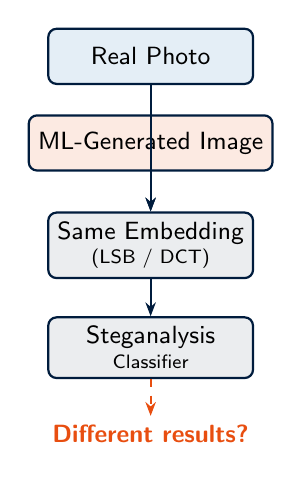
\begin{tikzpicture}[
  box/.style={draw=umdark,rounded corners=3pt,minimum width=2.6cm,minimum height=0.7cm,align=center,font=\small,thick},
  arr/.style={-{Stealth[length=5pt]},thick,umdark}
]
\node[box,fill=umlight!15] (real) at (0,3.0) {Real Photo};
\node[box,fill=umorange!12] (ml) at (0,1.9) {ML-Generated Image};
\node[box,fill=umdark!8] (embed) at (0,0.6) {Same Embedding\\[-2pt]{\scriptsize(LSB / DCT)}};
\node[box,fill=umdark!8] (detect) at (0,-0.7) {Steganalysis\\[-2pt]{\scriptsize Classifier}};
\node[font=\small\bfseries,text=umorange] (q) at (0,-1.8) {Different results?};

\draw[arr] (real.south) -- (embed.north);
\draw[arr] (ml.south) -- (embed.north);
\draw[arr] (embed.south) -- (detect.north);
\draw[arr,dashed,umorange] (detect.south) -- (q.north);
\end{tikzpicture}
\end{column}
\end{columns}
\end{frame}

% ============================================================
\section{Why This Study Matters}
% ============================================================

\begin{frame}{Why Should We Care?}
\small
\begin{columns}[T]
\begin{column}{0.46\textwidth}
{\color{umorange}\textbf{1. Security Implications}}
\begin{itemize}
\item If ML images are harder to steganalyze $\rightarrow$ adversaries exploit synthetic carriers
\item If easier to detect $\rightarrow$ new forensic opportunities
\end{itemize}

\medskip

{\color{umorange}\textbf{2. Timely \& Novel}}
\begin{itemize}
\item AI images are everywhere (social media, news, art)
\item \textbf{No systematic study} compares real vs.\ ML images as steganographic carriers under controlled conditions
\item De et al.\ (2022) touched this space but did not do a controlled comparison
\end{itemize}
\end{column}

\begin{column}{0.46\textwidth}
{\color{umorange}\textbf{3. Scientifically Interesting}}
\begin{itemize}
\item Generative models impose learned statistical regularities (GAN spectral peaks, diffusion noise patterns)
\item How do these interact with steganographic distortion?
\item Tests cross-domain classifier generalization
\end{itemize}

\medskip

{\color{umorange}\textbf{4. Practical Scope}}
\begin{itemize}
\item Well-defined, testable hypotheses
\item Clear experimental pipeline
\item Open-source tools + our own hardware
\item Quantitative results (AUC, accuracy, EER)
\end{itemize}
\end{column}
\end{columns}
\end{frame}

% ============================================================
\section{Research Questions}
% ============================================================

\begin{frame}{Research Questions}

\begin{block}{Primary Research Question}
\textit{Does the source of the carrier image (real human-photographed vs.\ ML-generated) affect the detectability of image steganography when using identical embedding methods and payload sizes?}
\end{block}

\vspace{0.3cm}

\begin{columns}[T]
\begin{column}{0.23\textwidth}
\begin{alertblock}{RQ1: Payload}
\small
How does payload size influence detectability across real and ML-generated images?
\end{alertblock}
\end{column}

\begin{column}{0.23\textwidth}
\begin{alertblock}{RQ2: Method}
\small
Do LSB (spatial) and DCT (freq-domain) behave differently by carrier origin?
\end{alertblock}
\end{column}

\begin{column}{0.23\textwidth}
\begin{alertblock}{RQ3: Encryption}
\small
Does encrypting the payload before embedding affect detectability?
\end{alertblock}
\end{column}

\begin{column}{0.23\textwidth}
\begin{alertblock}{RQ4: Cross-Domain}
\small
Do classifiers trained on real images generalize to ML-generated images, and vice versa?
\end{alertblock}
\end{column}
\end{columns}
\end{frame}

% ============================================================
\section{Experimental Setup}
% ============================================================

\begin{frame}{Experimental Pipeline}
\vspace{0.4cm}
\centering
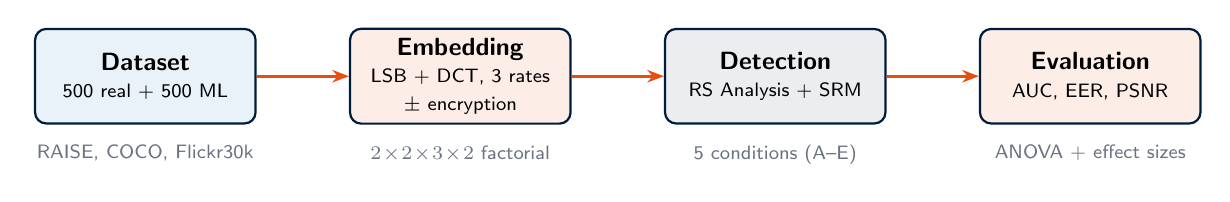
\begin{tikzpicture}[
  box/.style={draw=umdark,rounded corners=4pt,minimum width=2.8cm,minimum height=1.2cm,align=center,font=\small,thick},
  arr/.style={-{Stealth[length=6pt]},very thick,umorange}
]
\node[box,fill=umlight!12] (data) at (0,0) {\textbf{Dataset}\\[-1pt]{\scriptsize 500 real + 500 ML}};
\node[box,fill=umorange!10] (embed) at (4,0) {\textbf{Embedding}\\[-1pt]{\scriptsize LSB + DCT, 3 rates}\\[-1pt]{\scriptsize $\pm$ encryption}};
\node[box,fill=umdark!8] (train) at (8,0) {\textbf{Detection}\\[-1pt]{\scriptsize RS Analysis + SRM}};
\node[box,fill=umorange!10] (eval) at (12,0) {\textbf{Evaluation}\\[-1pt]{\scriptsize AUC, EER, PSNR}};

\draw[arr] (data) -- (embed);
\draw[arr] (embed) -- (train);
\draw[arr] (train) -- (eval);

\node[font=\scriptsize,text=umgray,below=4pt of data] {RAISE, COCO, Flickr30k};
\node[font=\scriptsize,text=umgray,below=4pt of embed] {$2\!\times\!2\!\times\!3\!\times\!2$ factorial};
\node[font=\scriptsize,text=umgray,below=4pt of train] {5 conditions (A--E)};
\node[font=\scriptsize,text=umgray,below=4pt of eval] {ANOVA + effect sizes};
\end{tikzpicture}

\vspace{0.6cm}

\begin{columns}[T]
\begin{column}{0.3\textwidth}
\centering
{\color{umorange}\textbf{4 Factors}}\\[4pt]
{\small Carrier $\times$ Method $\times$ Payload (3) $\times$ Detector}
\end{column}
\begin{column}{0.3\textwidth}
\centering
{\color{umorange}\textbf{Matched Pairs}}\\[4pt]
{\small Real photos matched to ML images by semantic content}
\end{column}
\begin{column}{0.3\textwidth}
\centering
{\color{umorange}\textbf{5 Train/Test Splits}}\\[4pt]
{\small Within-domain, cross-domain, and mixed}
\end{column}
\end{columns}
\end{frame}

% ---- Datasets ----
\begin{frame}{Datasets}
\begin{columns}[T]
\begin{column}{0.46\textwidth}
\begin{exampleblock}{Real Images (500 photos)}
\begin{itemize}
\item \textbf{RAISE}: High-quality RAW photos from DSLR cameras, diverse scenes
\item \textbf{COCO / Flickr30k}: Natural photographs, diverse content
\item Normalized: 512$\times$512 px, RGB, 8-bit PNG
\end{itemize}
\end{exampleblock}
\end{column}

\begin{column}{0.46\textwidth}
\begin{block}{ML-Generated Images (500 images)}
\begin{itemize}
\item \textbf{Stable Diffusion}: Latent diffusion, photorealistic text-to-image
\item \textbf{StyleGAN3}: GAN-based, well-characterized spectral artifacts
\item Same 512$\times$512, RGB, 8-bit PNG format
\end{itemize}
\end{block}
\end{column}
\end{columns}

\vspace{0.4cm}

\centering
{\small\color{umgray}\textbf{Matching protocol:}\enspace ML images generated from same semantic prompts as real image content\enspace$\cdot$\enspace Identical format specs\enspace$\cdot$\enspace Consistent mean luminance}
\end{frame}

% ---- Embedding ----
\begin{frame}{Embedding, Payload Rates \& Encryption}
\begin{columns}[T]
\begin{column}{0.46\textwidth}
{\color{umorange}\textbf{LSB Substitution}} {\small(spatial domain)}
\begin{itemize}
\item Replace $k$ least significant bits of pixel values
\item Pseudorandom pixel selection across RGB channels
\item High capacity, lower robustness
\end{itemize}

\bigskip

{\color{umorange}\textbf{DCT-Based Embedding}} {\small(frequency domain)}
\begin{itemize}
\item 8$\times$8 pixel blocks, QIM on mid-frequency DCT coefficients
\item Mirrors JPEG-domain steganography (F5 / JSteg)
\item Better imperceptibility, lower capacity
\end{itemize}

\bigskip

{\color{umorange}\textbf{Encryption (RQ3)}}
\begin{itemize}
\item AES-256 applied to payload before embedding
\item Tests whether payload structure affects detectability
\end{itemize}
\end{column}

\begin{column}{0.46\textwidth}
\vspace{0.3cm}
\centering
\small
\begin{tabular}{@{}lll@{}}
\toprule
\textbf{Level} & \textbf{LSB} & \textbf{DCT} \\
\midrule
Low      & $k\!=\!1$, 25\% px & 10\% coeff. \\
Medium   & $k\!=\!1$, 50\% px & 25\% coeff. \\
High     & $k\!=\!2$, 50\% px & 50\% coeff. \\
\bottomrule
\end{tabular}

\vspace{0.3cm}
{\small bpp = bits per pixel}
\end{column}
\end{columns}
\end{frame}

% ---- Cross-domain ----
\begin{frame}{Cross-Domain Conditions}
\vspace{0.2cm}
\centering
\small
\begin{tabular}{@{}cllp{7cm}@{}}
\toprule
& \textbf{Train on} & \textbf{Test on} & \textbf{What it tells us} \\
\midrule
\textbf{A} & Real    & Real    & Baseline: standard steganalysis performance \\
\textbf{B} & ML-gen  & ML-gen  & Is ML imagery inherently easier/harder to steganalyze? \\
\textbf{C} & Real    & ML-gen  & Can a ``real-trained'' detector catch ML-embedded stego? \\
\textbf{D} & ML-gen  & Real    & Can an ``ML-trained'' detector catch real-embedded stego? \\
\midrule
\textbf{E} & Mixed   & Both    & Does mixed training solve the domain gap? \\
\bottomrule
\end{tabular}

\vspace{0.4cm}

\begin{block}{Key Insight}
Conditions \textbf{C} and \textbf{D} directly test \textbf{RQ4} (cross-domain generalization).
Comparing \textbf{A} vs.\ \textbf{B} addresses the \textbf{primary RQ}.
\end{block}
\end{frame}

% ============================================================
\section{Hypotheses}
% ============================================================

\begin{frame}{Hypotheses}
\vspace{0.1cm}

{\color{umorange}\textbf{H1 -- Distributional Difference}}\quad ML images will show \textit{different} detectability due to learned statistical regularities (GAN spectral peaks, diffusion noise patterns, smoother textures).

\medskip

{\color{umorange}\textbf{H2 -- Payload Divergence}}\quad The gap between carrier types \textit{widens} at higher payloads. At low rates, both may be equally hard to detect.

\medskip

{\color{umorange}\textbf{H3 -- Method Sensitivity}}\quad DCT embedding will be \textit{more} sensitive to carrier origin than LSB, because DCT coefficients are directly shaped by the generative process.

\medskip

{\color{umorange}\textbf{H4 -- Cross-Domain Drop}}\quad Classifiers will lose \textbf{10--25\% AUC} when tested across domains, mirroring image deepfake detection findings.

\medskip

{\color{umorange}\textbf{H5 -- Asymmetric Transfer}}\quad Real$\to$ML transfer (C) will perform \textit{worse} than ML$\to$Real (D), because ML images' distinctive statistical profile masks learned artifacts.

\medskip

{\color{umorange}\textbf{H6 -- Encryption Effect}}\quad Payload encryption will not significantly affect detectability, since AES output is statistically similar to a pseudorandom bitstream.
\end{frame}

% ============================================================
\section{Literature Coverage}
% ============================================================

\begin{frame}{Literature Coverage}
\vspace{0.1cm}
\begin{columns}[T]
\begin{column}{0.46\textwidth}
{\color{umorange}\textbf{Image Steganography Surveys}}\\
{\small Petitcolas et al.\ (1999) -- Hussain et al.\ (2018)}

\medskip

{\color{umorange}\textbf{Image Steganalysis}}\\
{\small Westfeld \& Pfitzmann (1999) -- Chi-square attack\\
Fridrich et al.\ (2001) -- RS Analysis\\
Fridrich \& Kodovský (2012) -- Rich Models (SRM)}

\medskip

{\color{umorange}\textbf{Embedding Theory}}\\
{\small Holub et al.\ (2014) -- HILL/S-UNIWARD\\
Westfeld (2001) -- F5 algorithm}

\end{column}
\begin{column}{0.46\textwidth}

{\color{umorange}\textbf{ML Image Generation}}\\
{\small Rombach et al.\ (2022) -- Stable Diffusion\\
Karras et al.\ (2021) -- StyleGAN3\\
OpenAI (2023) -- DALL-E 3}

\medskip

{\color{umorange}\textbf{AI + Steganography (The Gap)}}\\
{\small De et al.\ (2022) -- AI image stego (closest prior work)\\
Duan et al.\ (2020) -- coverless GAN stego}

\medskip

{\color{umorange}\textbf{Deepfake Detection \& Datasets}}\\
{\small Wang et al.\ (2020) -- CNN-generated image detection\\
Corvi et al.\ (2023) -- diffusion model detection\\
RAISE, COCO, Flickr30k datasets}

\end{column}
\end{columns}
\end{frame}

% ============================================================
\section{Pros \& Cons}
% ============================================================

\begin{frame}{Pros \& Cons}
\begin{columns}[T]
\begin{column}{0.46\textwidth}
\begin{exampleblock}{Pros}
\begin{itemize}
\item \textbf{Clear research gap} -- no prior systematic controlled study
\item \textbf{Well-defined} -- testable hypotheses, quantitative metrics
\item \textbf{Runs locally} -- Stable Diffusion + StyleGAN3 on M4 Pro, no cloud GPUs
\item \textbf{Modular pipeline} -- independent stages, parallelizable
\item \textbf{Publishable angle} -- timely intersection of two active fields
\item \textbf{Better tooling than audio} -- mature image steganalysis baselines
\end{itemize}
\end{exampleblock}
\end{column}

\begin{column}{0.46\textwidth}
\begin{alertblock}{Cons / Risks}
\begin{itemize}
\item \textbf{6--7 weeks is tight} -- disciplined timeline needed
\item \textbf{Null result risk} -- carrier origin may show no effect
\item \textbf{Dataset size} -- 500 per carrier type; covers the main experimental conditions
\item \textbf{Scope creep} -- tempting to add more generation models
\item \textbf{DCT complexity} -- JPEG-domain embedding requires careful block-level implementation
\item \textbf{Matching difficulty} -- semantic matching of real vs.\ ML images is imperfect
\end{itemize}
\end{alertblock}
\end{column}
\end{columns}
\end{frame}

% ============================================================
\section{Feasibility \& Timeline}
% ============================================================

\begin{frame}{Feasibility \& Timeline}
\begin{columns}[T]
\begin{column}{0.48\textwidth}
{\color{umorange}\textbf{Hardware}}\enspace M4 Pro MacBooks (18--36\,GB unified memory)

\medskip

{\color{umorange}\textbf{Image generation}}
\begin{itemize}
\item Stable Diffusion: $\sim$3--5\,h for 250 images (MPS)
\item StyleGAN3: $\sim$2--3\,h for 250 images
\item Real images: download from RAISE/COCO
\end{itemize}

\medskip

{\color{umorange}\textbf{Detection (CPU-only)}}
\begin{itemize}
\item RS Analysis \& chi-square: seconds per image, no training
\item SRM + FLD: $\sim$30\,min total (scikit-learn, CPU)
\item \textbf{Total compute: $<$5\,h} (vs.\ days with neural nets)
\end{itemize}

\medskip

{\small All tools open-source: Python, NumPy, SciPy, scikit-learn, scikit-image}
\end{column}

\begin{column}{0.44\textwidth}
\vspace{0.1cm}
\centering
\small
\begin{tabular}{@{}cl@{}}
\toprule
\textbf{Week} & \textbf{Activity} \\
\midrule
1     & Data collection \& ML image generation \\
2     & Stego implementation (LSB + DCT $\pm$ AES) \\
3--4  & Classifier training (all conditions) \\
5     & Cross-domain experiments \& analysis \\
6     & Paper writing \& visualization \\
7     & Buffer / revision / submission \\
\bottomrule
\end{tabular}

\vspace{0.4cm}

\begin{block}{\small Parallelization}
\footnotesize
Wk 1--2: split data gen \& embedding\\
Wk 3--4: each member trains subset\\
Wk 5--6: analysis \& writing in parallel
\end{block}
\end{column}
\end{columns}
\end{frame}

% ============================================================
\section{Risk Mitigation}
% ============================================================

\begin{frame}{Risk Mitigation}
\vspace{0.1cm}
\small
\renewcommand{\arraystretch}{1.4}
\begin{tabular}{@{}p{3.8cm}p{9.5cm}@{}}
\toprule
\textbf{Risk} & \textbf{Mitigation} \\
\midrule
Null result & A null result \textit{is} a valid finding -- shows existing steganalysis generalizes well across carrier origins. Frame accordingly. \\
Dataset too small & Data augmentation (flips, crops, color jitter on cover images before embedding); target 500 total if time allows. \\
Semantic matching imperfect & Define matching as same semantic category (not same scene); document as a design choice. \\
DCT implementation & Start with LSB (simpler); use reference implementations (OpenStego); DCT as secondary. \\
Scope creep & Freeze design after Week 2; additional generation models go into ``future work.'' \\
\bottomrule
\end{tabular}
\end{frame}

% ============================================================
\section{Discussion}
% ============================================================

\begin{frame}{Discussion}
\vspace{0.2cm}
\begin{enumerate}
\item {\color{umorange}\textbf{Dataset size:}} 500 per carrier type (250 per model) -- extended from 300 to improve statistical power

\bigskip

\item {\color{umorange}\textbf{Generation models:}} Stable Diffusion + StyleGAN3 sufficient, or add DALL-E 3 as a third (API-based)?

\bigskip

\item {\color{umorange}\textbf{Division of labor:}} Proposed split --
  \begin{itemize}
  \item \textit{Data team} (2): dataset collection, ML image generation, normalization
  \item \textit{Stego team} (2): LSB + DCT implementation, AES encryption, embedding pipeline
  \item \textit{Classification team} (2): classifier training, evaluation, statistics
  \end{itemize}

\bigskip

\item {\color{umorange}\textbf{Matching definition:}} Same scene vs.\ same semantic category -- which is more defensible?

\bigskip

\item {\color{umorange}\textbf{Should we proceed with this topic?}}
\end{enumerate}
\end{frame}

% ============================================================
% CLOSING
% ============================================================

\begin{frame}[plain]
\vfill
\begin{center}
{\color{umorange}\rule{0.3\textwidth}{2pt}}\\[16pt]
{\LARGE\bfseries\color{umdark}Thank you}\\[10pt]
{\large\color{umgray}Questions \& Discussion}\\[20pt]
{\small\color{umgray}Full proposal PDF and reference review available for detailed reading.}\\[16pt]
{\color{umorange}\rule{0.3\textwidth}{2pt}}
\end{center}
\vfill
\end{frame}

\end{document}
